%%
%% This is file `skeleton.tex',
%% generated with the docstrip utility.
%%
%% The original source files were:
%%
%% nuthesis.dtx  (with options: `skeleton')
%% 

%%
%% For common degrees, you can use the class options:
%% phd, edd, ms, ma
%% phd is the default
\documentclass[print]{nuthesis}
\begin{document}
%% Start formatting the first few special pages
%% frontmatter is needed to set the page numbering correctly
\frontmatter

\title{Enabling Distributed Scientific Computing on the Campus}
\author{Derek Weitzel}
\adviser{Dr. David Swanson}
\adviserAbstract{Someone}
\major{Computer Science}
\degreemonth{May}
\degreeyear{2014}
%%
%% For most people the defaults will be correct, so they are commented
%% out. To manually set these, just uncomment and make the needed
%% changes.
%% \college{Your college}
%% \city{Your City}
%%
%% For most people the following can be changed with a class
%% option. To manually set these, just uncomment the following and
%% make the needed changes.
%% \doctype{Thesis or Dissertation}
%% \degree{Your degree}
%% \degreeabbreviation{Your degree abbr.}
%%
%% Now that we know everything we need, we can generate the title page
%% itself.
%%
\maketitle
%%
%% You have a maximum of 350 words for your abstract, which includes
%% your title, name, etc.
%%
%% Required
\begin{abstract}

\end{abstract}

%% Optional
%% \begin{copyrightpage}
%% \end{copyrightpage}

%% Optional
%% \begin{dedication}
%% \end{dedication}

%% Optional
%% \begin{acknowledgments}
%% \end{acknowledgments}

%% Optional
%% \begin{grantinfo}
%% \end{grantinfo}
%% The ToC is required
%% Uncomment these if need be

%% The ToC is required
\tableofcontents
%% Uncomment these if need be
\listoffigures
\listoftables
%%
%% ``Real'' beginning of the document.
%% mainmatter is needed to set the page numbering correctly
%%   mainmatter is needed after the ToC, (LoF, and LoT) to set the
%%   page numbering correctly for the main body
\mainmatter

%% Thesis goes here

\chapter{Introduction}








\chapter{Related Work}
\label{chapter:relatedwork}

\section{Distributed Batch Systems}


Several batch systems and grid schedulers are able to schedule tasks on execution resources.  Examples of cluster schedulers that are frequently used are PBS \cite{pbstorque}, \mbox{HTCondor} \cite{litzkow1988condor}, and SLURM \cite{yoo2003slurm}.  Each scheduler is very good at resource management within a single administrative domain.  But, each of these resource managers have very limited ability to send processing to remote resources, which are typically under a separate administrative domain.  PBS and SLURM can send jobs between clusters that run the same schedulers.  HTCondor also has the ability to send processing to other clusters running HTCondor and it can also transform jobs to the language of other schedulers such as PBS and SLURM.

Grid schedulers have become more popular as the number of resources has increased.  Examples of grid schedulers are OSGMM \cite{website:osgmm} and GlideinWMS \cite{sfiligoi2008glideinwms}.  These schedulers are able to send jobs to remote resources using grid protocols.  OSGMM performs a direct grid submission to the remote resources using the GRAM  \cite{foster1999globus} interface.  GlideinWMS also submits to the GRAM interface of the cluster, but provides an overlay of HTCondor daemons on top of remote resources.  The overlay presents a consistent HTCondor interface to the computing resources for ease of use.  


\section{Distributed Storage Access}

Distributed file systems have long had their own storage access methods.  An example of this is Hadoop \cite{white2012hadoop}, a popular distributed file and processing system.  The only method to access Hadoop storage is through the Hadoop protocol.  On the Open Science Grid, the primary access methods are through file system independent middleware such as the Storage Resource Manager (SRM) \cite{shoshani2002storage} and XRootd \cite{dorigo2005xrootd}.  They provide a translation layer from system independent grid protocols and security mechanisms to the underlying storage system, such as Hadoop.  The Storage Resource Manager (SRM) is a previously popular protocol to access remote distributed filesystems.  It is a standardized protocol that allows remote, distributed access to large storage with APIs to balance transfers among many data servers.


Beyond storage access methods are storage schedulers.  These schedulers do not define a protocol to access the storage, rather they coordinate the access.  NeST \cite{bent2002flexibility} is a software-only grid aware storage scheduler.  It supports multiple transfer protocols into a storage device, including GridFTP \cite{allcock2005globus} and NFS \cite{walsh1985overview}.  Further, it provides features such as resource discovery, storage guarantees, quality of service, and user authentication.  It is layered over a distributed filesystem to provide access to it.  NeST functions as the interface and access scheduler for a storage device.  Features such as the storage guarantees and quality of service require NeST to be the only interface into the storage device, a very rare feature in today's grid storage.  Today's storage elements, such as the 3PB storage at Nebraska, include multiple interfaces to access the storage element.  Nebraska runs at least four \cite{attebury2009hadoop} methods of accessing and modifying storage, SRM \cite{shoshani2002storage}, GridFTP, XrootD, and Fuse \cite{szeredi2010fuse} mounted Hadoop.  All of these methods are required for compatibility with different access patterns and clients.  NeST could implement each of these protocols, but it would be extremely difficult to manage the storage centrally.  For example, Fuse is mounted on all 300 worker nodes.  The GridFTP and XrootD servers run on 10's of servers, with an aggregate bandwidth of 10Gbps.  Scaling quality of service and storage allocation / enforcement across all of these access methods would likely prove impossible.



\section{Data Transfer Mechanisms}

A popular consumer transfer method, Bittorrent, has been used for data transfer in computational grids by Wei et al \cite{wei2005collaborative, wei2005scheduling, wei2007towards}.  It has been shown to improve data transfer speeds when compared to traditional source and sink transfer methods, in this case FTP \cite{postel1985file}, which is very similar in architecture to GridFTP, a grid enabled FTP protocol.  The researchers did not compare performance of the bittorrent protocol when compared to modern grid transfer techniques, such as using HTTP local caching.  Further, the authors do not test bittorrent transfers across network partitions that are common on the grid.  For example, a worker node from one cluster may not be able to communicate directly with another cluster.  Therefore, bittorrent may not work between clusters, but will work inside clusters.

Globus online \cite{foster2011globus} is a web interface for transferring files between sites and sharing data with other users.  It offers an intuitive web interface for bulk transfers between endpoints.  It only supports the gridftp \cite{allcock2005globus} transfer protocol, and requires GridFTP implementations at all endpoints.

Stork \cite{kosar2004stork} is a data placement scheduler.  It can schedule data placement and transfers to and from remote storage systems.  Stork is innovative in that it treats data transfers similar to jobs.  It will queue transfers, and checks for proper completion of the transfers.

Kangaroo \cite{thain2001kangaroo} is another storage scheduler multi-level file access system.  It allows for multiple levels of staging in order to send job output back to a storage device.  It can do this by asynchronously staging data through multiple storage devices on it's path to the destination filesystem.  The Kangaroo system only addresses output data.

\section{Data Management}

There have been previous policy frameworks for distributed storage.  These frameworks have largely been designed to move data between few large filesystems.  Therefore, the interactions are rare, but could make significant changes to the system.  In contrast, the CacheD's have frequent interactions with other agents, but each one has a minimal impact on the entire system.

Data management is different from data transfer and access in that it provides services on top of the file systems, such as meta-data storage and search capabilities.  An example of a Data management service is iRods \cite{rajasekar2010irods}.  It provides meta-data storage and querying, and rule based placements.  Further, it can handle transfers to storage resources.

DQ2 \cite{branco2008managing} and Phedex \cite{rehn2006phedex} are production transfer services for the Atlas and CMS physics experiments, respectively.  They are used to manage distributed transfers to and from sites inside the collaborations.  Additionally, they have had databases built on top of them that provide features such as combining files into datasets for easier bulk transfer management.  Both were designed for their experiments, and therefore would be very difficult to generalize for outside users.

\begin{figure}[ht!]
	\centering
	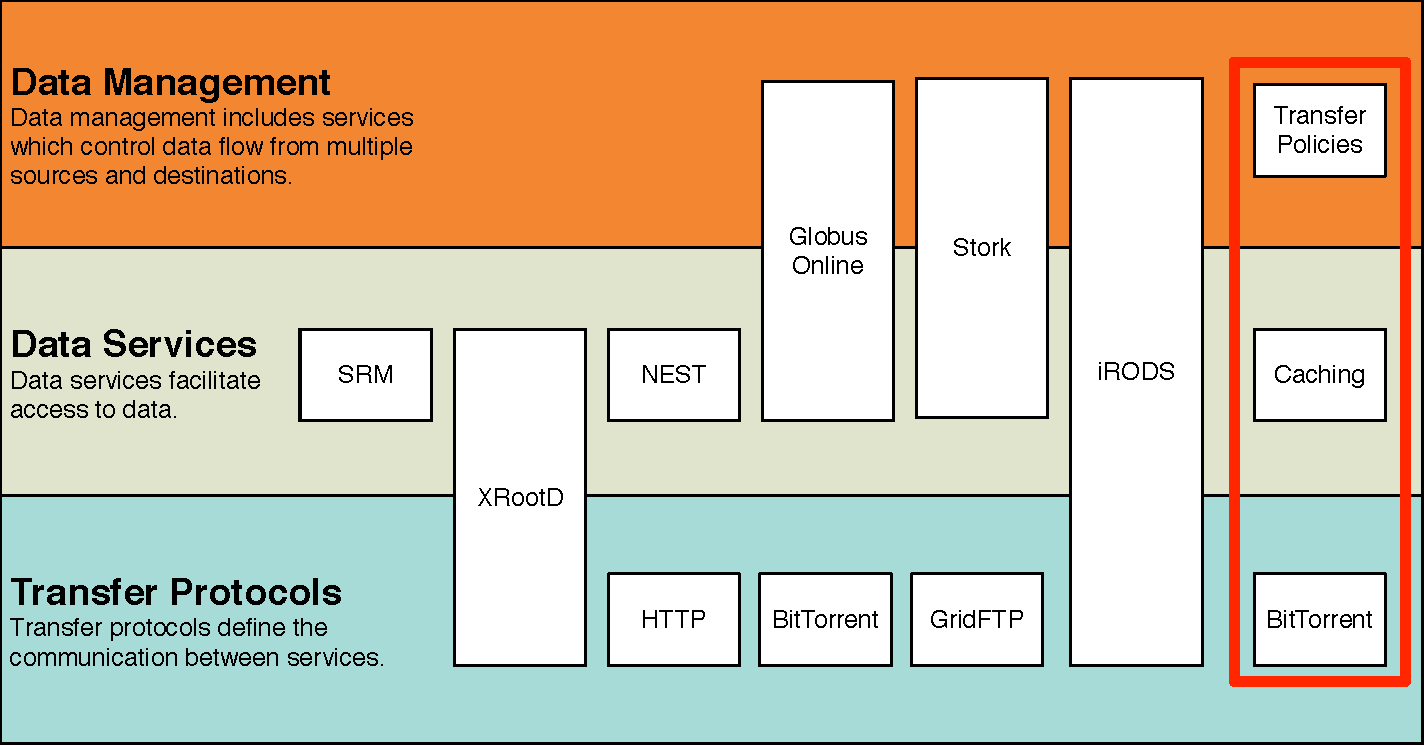
\includegraphics[width=\textwidth]{images/BackgroundStorageDiagram2.pdf}
	\caption{Background on storage technologies}
	\label{fig:backgroundstorage}
\end{figure}


\section{State of Practice in Campus Computing}
%TODO: write state of practice in campus computing





\chapter{Campus Job Distribtuion}
In this chapter I will discuss Bosco.

\chapter{Campus Storage Access}
In this chapter I will discuss
\label{chapter:campusdata}

\section{Introduction}

In the previous chapter, Chapter \ref{chapter:coordinatingstorage}, I discussed the HTCondor CacheD.  In this section, I will discuss the policy framework that allows the CacheD to represent heterogeneous resources on campus or cyberinfrastructure resources.  The CacheD's policy framework inserts itself whenever it interacts with another CacheD.  This policy framework allows the CacheD to act as an independent agent within the distributed system.

\begin{description}
	\item[Choosing a Replication Target] - A CacheD that is the origin to a cache may choose to proactively replicate to other CacheDs.  Choosing a replication target requires matching the cache's requirements with that of the target CacheD's.
	\item[Accepting Cache Replication] - A CacheD must decide if it can accept a cache when it receives a replication request.  This decision is based on it's own policy, as well as attributes of the incoming cache.
	\item[Transfer Method] - The transfer method for a cache to be replicated is chosen after a cache has been accepted.  This is a prioritized list of acceptable transfer methods for the cache.

\end{description}

\section{Policy Language}
The policy language used by the CacheD is the HTCondor ClassAds \cite{raman1998matchmaking}.  ClassAds offer the flexibility to both describe resources with attributes.  A ClassAd is a set of key value attributes.  The values can be numbers, strings, lists of strings, or boolean expressions.

% example CacheD ClassAd
\begin{figure}
\begin{lstlisting}[breaklines=true, breakatwhitespace=true,frame=single]
CachedServer = true
Machine = "red-foreman.unl.edu"
LastHeardFrom = 1433790880
UpdatesTotal = 8660
Name = "cached-22815@red-foreman.unl.edu"
CondorPlatform = "$CondorPlatform: X86_64-ScientificLinux_6.5 $"
UpdatesHistory = "0x00000000000000000000000000000000"
UpdatesLost = 0
TotalDisk = 6769920
UpdateSequenceNumber = 32307
UpdatesSequenced = 8659
MyAddress = "<129.93.239.170:11000?noUDP&sock=22815_fb39>"
AuthenticatedIdentity = "dweitzel@unl.edu"
DetectedMemory = 7807
Requirements = MY.TotalDisk > TARGET.DiskUsage
CondorVersion = "$CondorVersion: 8.3.1 Dec 22 2014 BuildID: UW_development PRE-RELEASE-UWCS $"
DetectedCpus = 2
DaemonStartTime = 1431839398
CurrentTime = time()
MyCurrentTime = 1433790880
\end{lstlisting}
\caption{CacheD ClassAd Example}
\label{lst:cachedclassad}
\end{figure}

Figure \ref{lst:cachedclassad} shows an example of a CacheD's ClassAd.  The attributes describe the CacheD daemon and the host it runs on.  For example, the \texttt{DaemonStartTime} is a representation of when the daemon started.  \texttt{TotalDisk} describes how much disk is available on the host that the CacheD is running.

% How matching works
Matching of ClassAds is done by comparing attributes between 2 sets of ClassAds.  The attribute \texttt{Requirements} takes a special meaning when matching two ClassAds.  The 
texttt{Requirements} attribute is a boolean expression that is evaluated in the context of both the current ClassAd and the matching ClassAd.  In the example in Figure \ref{lst:cachedclassad}, the CacheD's ClassAd would only match another ClassAd if the expression \texttt{MY.TotalDisk > TARGET.DiskUsage}.  This means that the CacheD will only accept caches that are smaller in size than the available disk on the host.  \texttt{MY} and \texttt{TARGET} refer to the current ClassAd and the matching ClassAd, respectively.


The \texttt{Requirements} attribute in Figure \ref{lst:cachedclassad} references other attributes in both the current ClassAd and the matching ClassAd.  Attributes can reference other attributes in order to form strings, lists, or boolean expressions.  In this example, the \texttt{Requirements} attribute references other attributes in order to create a boolean expression.


% Extending policy language
The ClassAd describing the CacheD can be extended by using the CacheD Cron mechanism.  The CacheD Cron executes an external program in order to collect statistics and reports the results in the CacheD's ClassAd.  These statistics can then be used to better describe either the daemon or the host machine.  A example of using the CacheD Cron is to collect the IO operations per second that a host is able to complete.  This information can be used to better match caches with machine which can run the applications, which is described in the sections below.


\section{Choosing a Replication Target}
% when it is used, and by who

% What is it matching against

% What if it doesn't match

% What if it does match


\section{Accepting Cache Replication}
% When it is used, and by who

% Special attributes

% 


\section{Transfer Method}

% List formation

% Negotiating preferences



\section{Measuring Storage}
In order to provide matchmaking for resources, the resources need to be accurately described and advertised.  This will require measuring the storage capabilities and capacity of the resources and advertising those attributes to the matchmaking service.

The measurements must be performed on the execution target as well as against the storage targets.  The execution targets will measure the storage capabilities in order to determine if the jobs can run.  The storage targets will be measured in order to determine the number of jobs that can be run against the target.


\subsection{Ranking Storage}
In order to find the most ideal resource for a job, the resources need to be ranked.  The simplest is a greedy approach where the resources are simply ranked by their benchmark speeds.  Additionally, they should only be ranked on the attributes requested by the job, i.e. if the job is only requesting X iops, then only rank resources on the IOPS available.

It is not immediately clear how the ranking should work.  If we assume that the user accurately describes their application needs, then we can pack the jobs onto resources by placing the job on the resource that meets the IOPS requirements, but has the least amount of IOPS remaining.  This will be an area of research to compare scheduling techniques on execution resources when considering their storage capabilities.


\section{Data Movement}
We will consider three different types of data.  The input data, output data, and the job sandbox.  The job sandbox is the environment from which the job will run.  The sandbox is important since the user designs their job to run in this sandbox, and it must be maintained in order for the job to run.  Also, the sandbox is shared input data that multiple executions of the job can utilize.

The sandbox is a set of files that must be present when the job begins execution.  For example, a sandbox may contain:
\begin{itemize}
\item The executable that the job will run.
\item Libraries necessary for the executable to properly function.
\item Shared input files such as parameter files or calibration data.
\end{itemize}

Some input data could be unique per job, therefore will be considered separately from the job sandbox.  Shared data between many executions can benefit from caching, where unique input data cannot benefit from caching.

Data for each job can be categorized as either shared, unique, private shared, or private unique.

\subsection{Categorizing Data}
% Describe shared data

\begin{table}
\begin{tabular}{l | l | l }
& Public & Private \\ 
\hline
Shared & Executables and Libraries & Personal identifying information \\ 
\hline
Unique & Input parameters & BLAST Query files \\
\hline
\end{tabular}

\end{table}

In order to better describe how data should be moved, we must categorize the data as shared or unique, private or non-private.  This creates a 2x2 matrix of possibilities of data.  Below, we define each of these categorizations.  Each of these categories comes with its own restrictions on how the data may be moved, and how it is presented to the user.

Shared data is data that is the same for multiple jobs in a job set.   In many cases, the majority of the files in the job sandbox can be considered shared data.  Examples of shared data are job executables and libraries.  

Frequently the job executables are the same for a large number of jobs.  Since the executables are the same, contextualization of the job is done through other methods, such as arguments or parameter files.  An example application that would use the same executables and libraries are Monte Carlo \cite{binder2010monte} simulations.  In these applications, the executables are the same for every job, each job is given a unique identifier which is used for the starting condition for the random generation.

Experimental data could also be shared between multiple jobs in a job set.  This can include common input data such as databases or condition data.  For example, BLAST \cite{altschul1990basic} jobs require a database of sequences of proteins which are then matched with specific queries.  The database is typically the same for a large number of queries.  

% May go into introduction
Many optimizations may be done to transfer shared data.  For example, people have used caching \cite{blumenfeld2008cms} the shared data per site.  Others have experimented using group transfer protocols such as Bittorrent \cite{cohen2008bittorrent} to distribute the shared data \cite{wei2005collaborative}.

% unique data
Data which is different for each job we define as unique data.  The unique data may be small things such as parameter files.  Or they may be large, such as sections of a database to search.  Unique data is defined as data which would not benefit from shared transfer, i.e., no other job needs the same data.

For our consideration, data which is not the same for every job in a job set, but is shared between jobs in a subset of the jobs will be considered shared data.

% private versions of shared and unique
We define private data as data which the user wants to prevent others from viewing.  The level of privacy requested by a user could determine how it can be enforced.  It could be enforced through authenticated access, encrypted data transfers, or both.  In most cases, authenticated data access is sufficient.

Private versions of shared and unique data cannot use the same optimization as public data.  For example, the data could not be transferred using a caching daemon if authenticated access is required.   Transferring data unauthenticated, even encrypted, is dangerous due to susceptibility to brute force.


After finding a resource to run on, the job sandbox and input data must be transferred to the remote host.  In order to do this, the remote execution host and the submitter must negotiate how to get the data there.  For example, does the remote host have access to the same NFS server?  Can it mount it?

\section{Description for these items}
Logically, we can separate these items into 2 categories
\begin{itemize}
\item Requirements for the application
\item Acceptable methods of data movement
\end{itemize}

The users must specify these items in the description of their jobs.  No consensus language for these specifications currently exists.  

The language for the requirements will be similar to the current specifications for memory and cpu.  The user will request certain storage parameters, and machines will need to provide these metrics just as they do now with cpu and memory.

The acceptable methods for data movement can either be specified by the user, or by the submitting system.  The system can stage the data to a third party, which will then be used for the transfer to the execution target.  This can be especially useful if multiple jobs use the same input data, a useful example of this is HCC�s use of LVS \cite{zhang2000linux} to serve common files on the OSG.  The server could automatically choose to use HTTP to transfer the files, especially since there are many common files, and the files would be cached on the remote sites using normal HTTP proxy caches.

%Another possible scenario is when starting a job on Amazon EC2.  If it is a virtual machine job, then input data could be created as a CD drive, or a block device, and input into the machine using the block device as input storage.

\section{Policy language for matchmaking storage}
The goal is to enable the user to describe their application to the scheduler in such a way that the scheduler can make intelligent decisions on:
\begin{itemize}
\item If the application can run on the pool
\item Where is the ideal location for the job to run
\item How to get the data to and from the application
\end{itemize}

% An example policy language for a job is:

\section{User Scenario}

A user creates their submit file and specifies their data.  The above policies will be matched to syntax in the submit file.  The syntax is shown in Listing \ref{lst:inputsyntax}.  We illustrate a shared, non-private case using a BLAST database, and a unique private file with the BLAST queries in Listing \ref{lst:blastsyntax}.  

\begin{figure}[h!]
\centering
\begin{lstlisting}[frame=single,caption={Input Syntax},captionpos=b,label={lst:inputsyntax}] 
{shared|unique}_{public|private}_input = <file1>,<file2>,...
\end{lstlisting}
\end{figure}



\begin{figure}[h!]
\centering
\begin{lstlisting}[frame=single,caption={Blast input syntax},captionpos=b,label={lst:blastsyntax}]
shared_public_input = blast_database.fasta
unique_private_input = queries
\end{lstlisting}
\end{figure}


The blast database is public, so there is no need to encrypt or authenticate access to the database.  Further, the database is shared between all executions of the job. The \texttt{queries} may contain personal identifiable information, and are therefore private and need authenticated access control in order to access the data.  

When the job begins, it will be guaranteed to have the files \texttt{blast\_database.fasta} and \texttt{queries} available to it.  The job framework will decide on the method of transfer and transient storage based on negotiation between the user specified syntax, the worker node, and the submit node.


\section{Defining Storage Target}
In this section, we define storage based on it�s capabilities:
\begin{itemize}
\item The total space available for an application or set of applications to store data.
\item The bandwidth available to the storage target.
\item The IOPS available to read / write to the storage (more applicable to local storage).
\item Access Protocol
\end{itemize}

Therefore, when mentioning storage, we must specify or estimate or discover all of these attributes.






%\section{Another Method for Data Transfer}
%In addition to the above methods for transferring data to remote worker nodes, and specifying storage parameters, we can also provide another method for getting data to worker nodes that will better fit the current state of clusters and cyberinfrastructure.  The proposed methods is a dynamic deployment of a storage federation.  This can be done across a single cluster, across many clusters, or over an entire national infrastructure such as the OSG.

%This new method for data transfer relies on peer to peer transfers.  Data is transferred from it�s peer rather than from a single host.  As with all peer to peer systems, the benefits from this method include decreasing the required bandwidth from any single source.  As well as lower latency transfers.


\chapter{Coordinating Campus Storage and Computation}



%% backmatter is needed at the end of the main body of your thesis to
%% set up page numbering correctly for the remainder of the thesis
\backmatter

%% Start the correct formatting for the appendices
\appendix

%% Appendices go here (if you have them)

%% Bibliography goes here (You better have one)
%% BibTeX is your friend

\bibliographystyle{plain}
\bibliography{DerekWeitzelDissertation}

%% Index go here (if you have one)
\end{document}

\endinput
%%
%% End of file `skeleton.tex'.
